\section{Appendix}
\begin{figure*}[h]
    \centering
    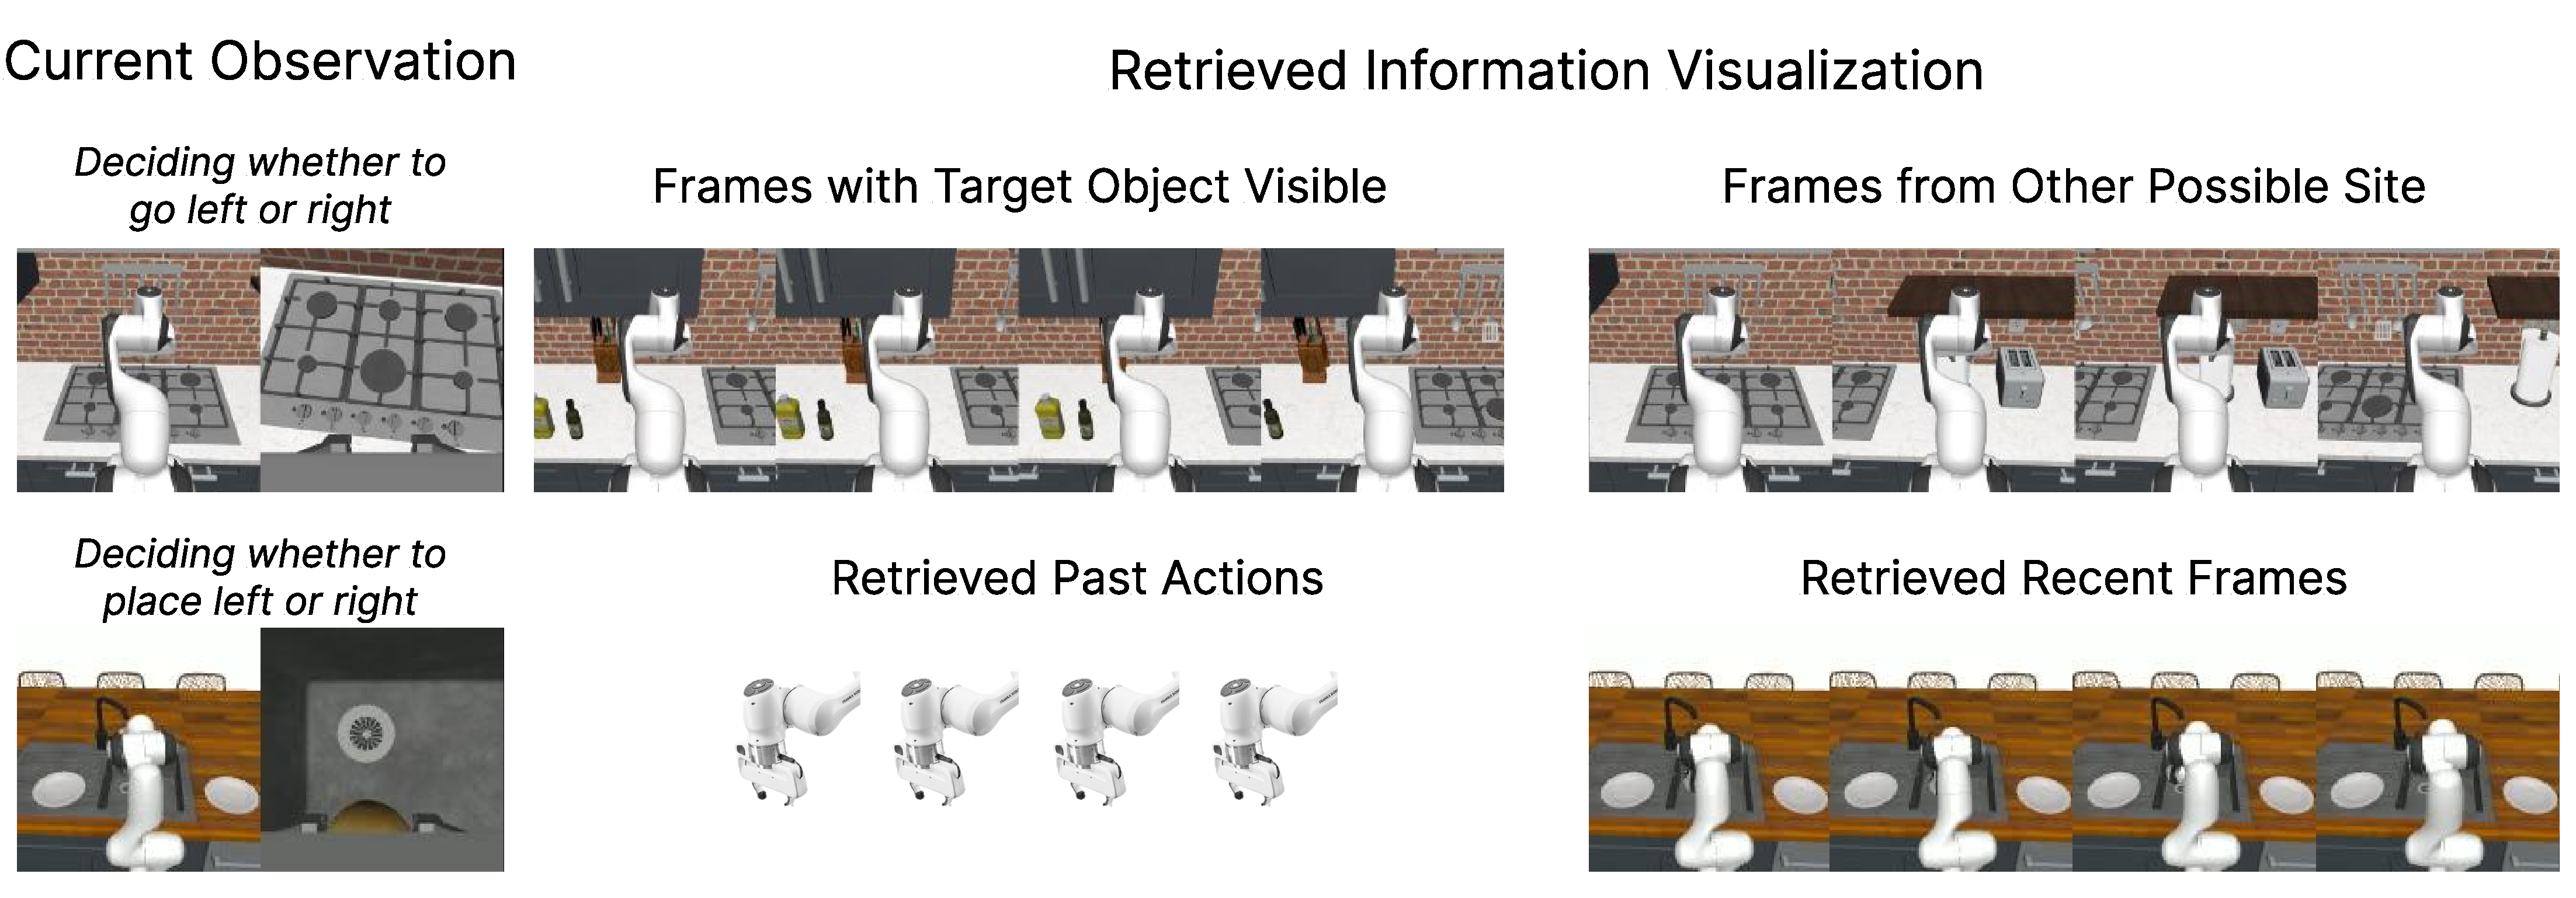
\includegraphics[width=\textwidth]{figures/retrieval_viz.pdf}
    \caption{Qualitative visualization of retrieved memory for two decision points. Left: current observations where the robot must choose a movement direction based on past information. Right: retrieved frames and action embeddings used for decision-making.}
    \label{fig:retrieval-viz}
    \vspace{-0.5em}
\end{figure*}
\subsection{Qualitative Analysis of Retrieved Information}\label{sec:app:retrieved_info_vis}
Qualitative examples are shown in Fig.~\ref{fig:retrieval-viz}. In the top example (Retrieve Object), the robot must choose a navigation direction based on where the target object was observed earlier in the episode. In the bottom example (Return to Same Container), the robot must place an object back into the correct container based on which container it was picked up from previously.

We notice that the policy retrieves heterogeneous and complementary information: for Retrieve Object (top, navigation), it retrieves both, frames where the target object (olive oil) was visible and frames from other locations where the target object is usually found but not currently placed; for Return to Same Container (bottom, manipulation), it retrieves both past actions and earlier frames that encode the object's original container and subgoal progress (`picked-up' vs. `placed').

This behavior goes beyond what simple, human-designed memory features (e.g., storing only frames where the object is visible) may capture. Together with the quantitative gains over hand-designed features  (Table~\ref{tab:sim_all}), these qualitative results suggest that learning what to retrieve directly from data with \ourmethod{} is more effective than manually specifying what to store, particularly for long-horizon, partially observable tasks.

\subsection{Qualitative Visualization of Generated VQA Data}\label{sec:app:vqa_viz}
We visualize examples of the generated VQA supervision used to train retrieval in Fig.~\ref{fig:qa_examples}. 
The questions probe different types of information, e.g., object locations, counts, and long-horizon task progress. 
These examples demonstrate that the generated VQA data provides diverse, task-relevant supervision for guiding memory retrieval. 
\subsection{Qualitative Visualization of Spurious Correlations}\label{sec:app:spurious_vis}
\begin{figure*}[t]
    \centering
    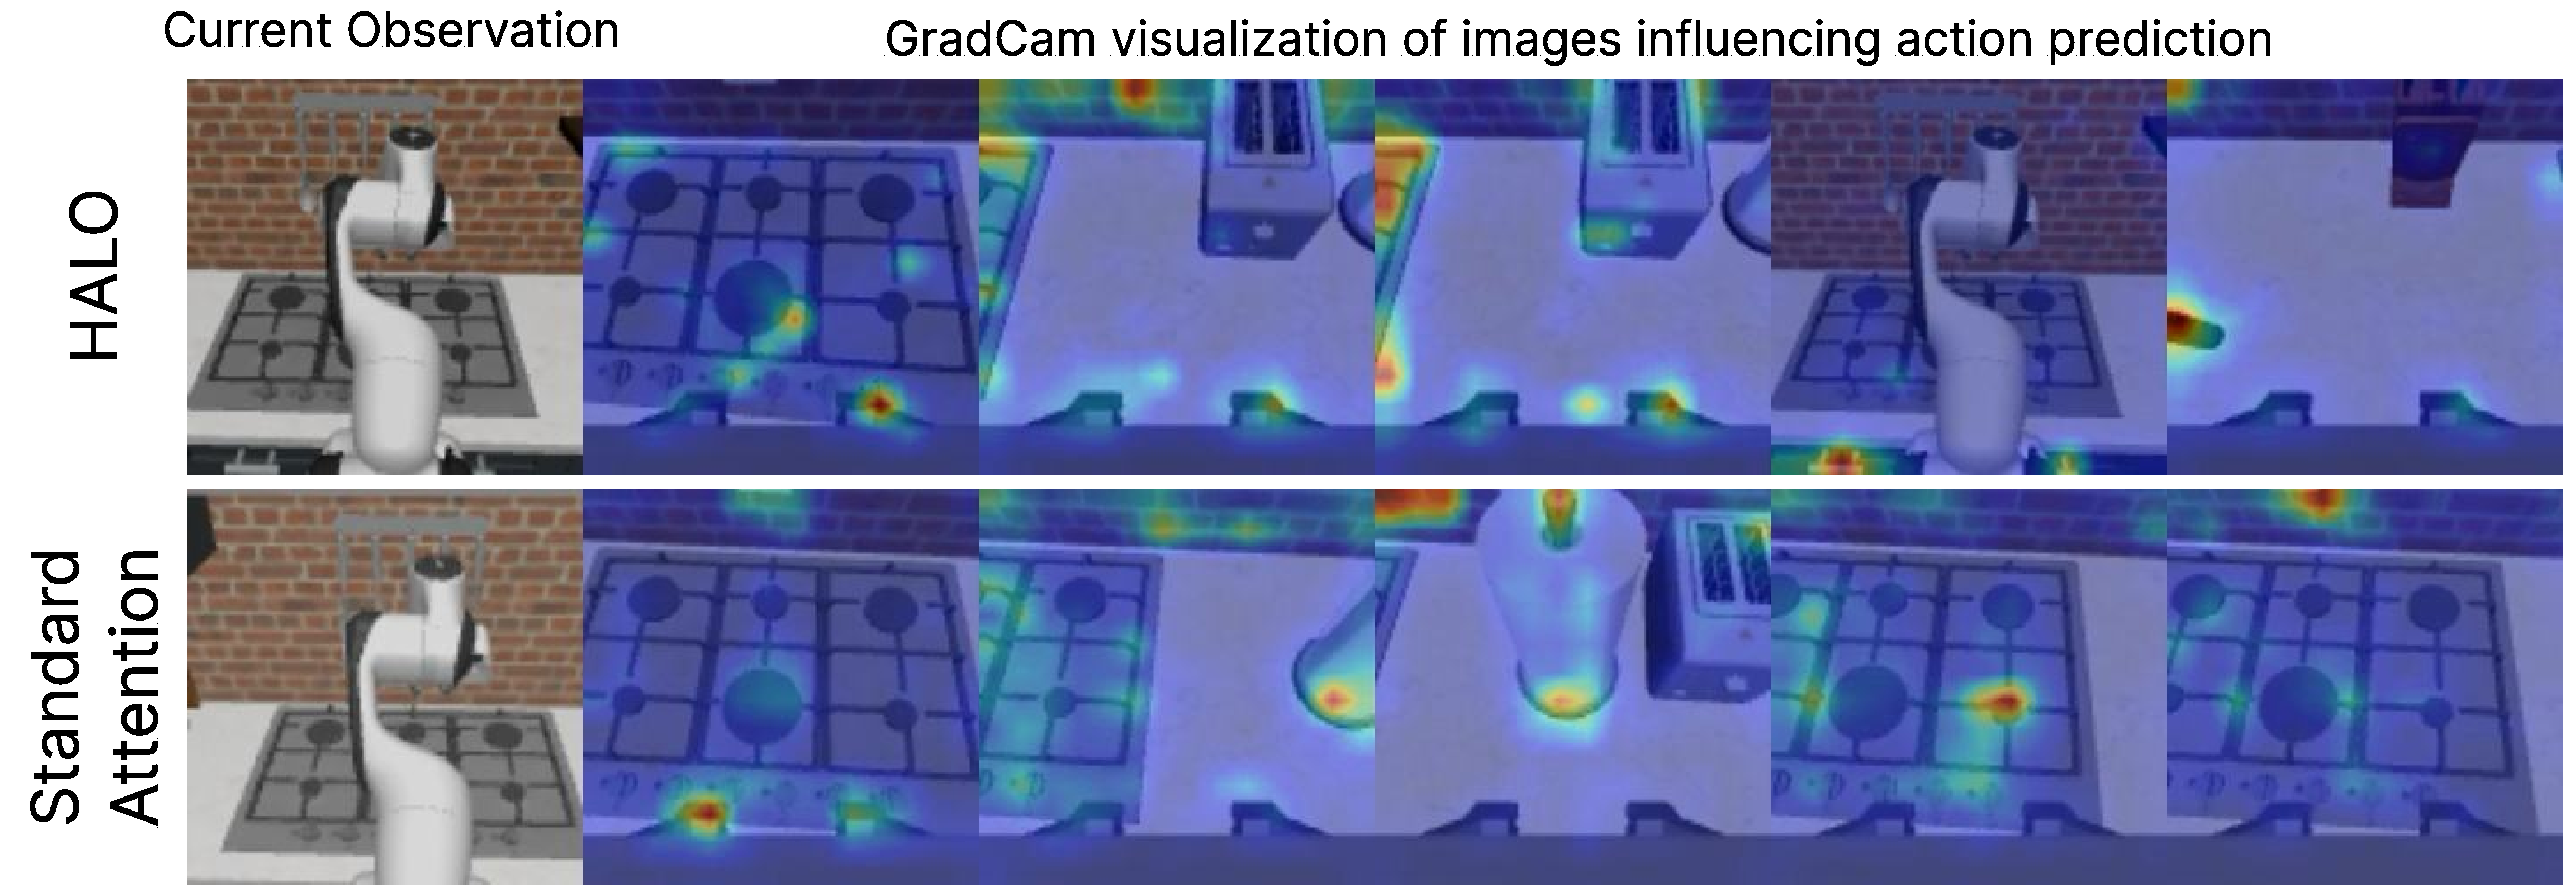
\includegraphics[width=0.98\textwidth]{figures/gradcam.pdf}
    \caption{Grad-CAM-style visualizations of image regions from history influencing action prediction. \textbf{Top:} \ourmethod{} focuses on the target object location (top-rightmost). \textbf{Bottom:} Without VQA supervision (standard Transformer), distractors may spuriously influence the action prediction (e.g., tissue roll position).}
    \label{fig:gradcam_viz}
\end{figure*}
We provide qualitative visualizations of image regions from the observation history that most influence the action prediction, following a GradCAM-style method~\cite{gradcam}.
A comparison between \ourmethod{} and the standard Transformer offers qualitative insight into spurious correlations that may influence action prediction in the absence of VQA supervision.

As shown in Figure~\ref{fig:gradcam_viz}, \ourmethod{} focuses more strongly on task-relevant target objects (e.g., the olive oil bottle), whereas the standard Transformer exhibits sensitivity to irrelevant distractors (e.g., the tissue roll position).
Together with the quantitative results in Table~\ref{tab:rw_all}, these visualizations suggest that adding VQA supervision reduces reliance on spurious visual correlations.
\subsection{Quantitative Analysis of Model Drift Errors}\label{sec:app:model_drift}
% \begin{figure}[th!]
%     \centering
%     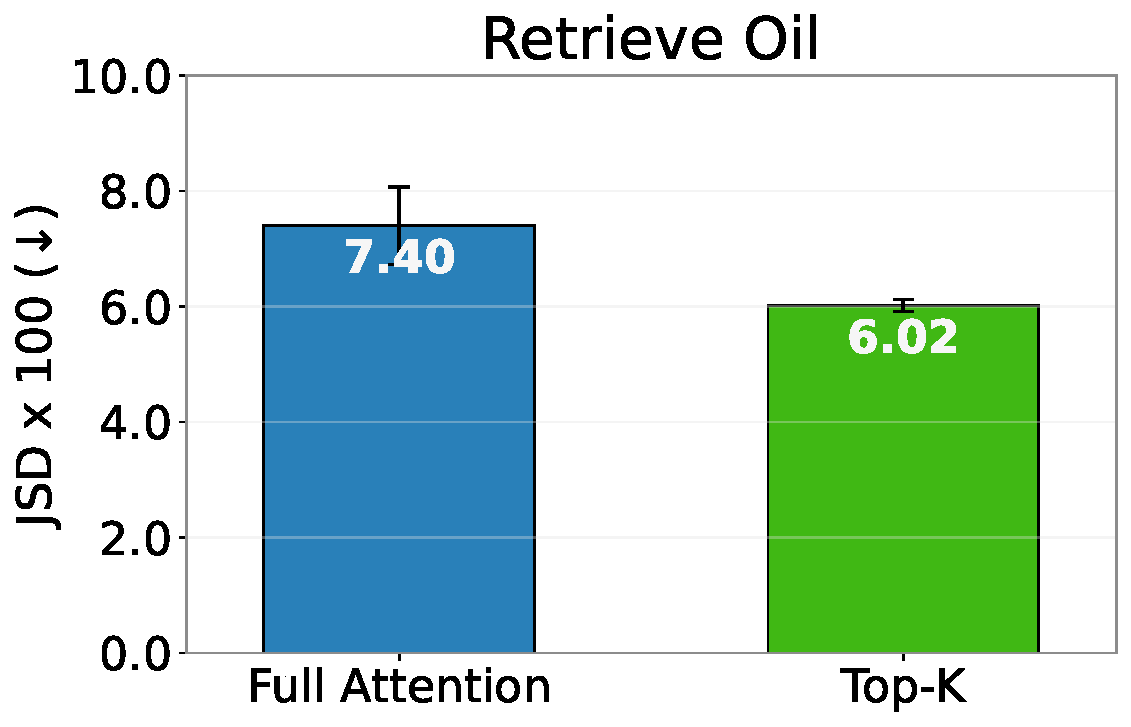
\includegraphics[width=0.95\columnwidth]{figures/JSD_bar_plot.pdf}
%     % \caption{.}
%     \label{fig:jsd_action}
%     \vspace{-0.5em}
% \end{figure}
{
\centering
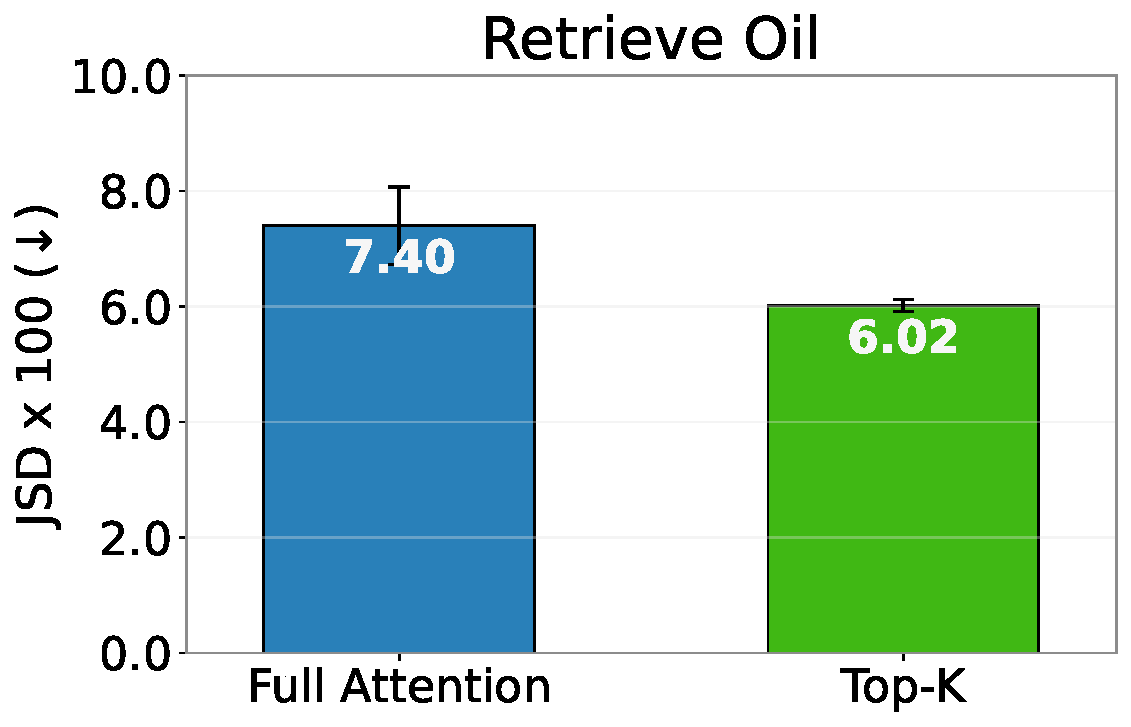
\includegraphics[width=0.80\columnwidth]{figures/JSD_bar_plot.pdf}
\label{fig:jsd_action}
}
\\
To quantify drift from expert behavior, we measure the distance between the policy's action distribution during rollouts and the expert's action distribution from teleoperated demonstrations. Both rollouts and expert trajectories are evaluated from identical initial environment configurations, using privileged resets in simulation to isolate differences attributable to the learned policy rather than to initial-state variation.

We quantify action distribution drift using the Jensen-Shannon divergence (JSD), a symmetric and bounded measure of discrepancy between probability distributions. For each task, we aggregate actions from rollouts and the corresponding expert demonstrations. Since actions are continuous, we discretize each action dimension into fixed bins and construct normalized histograms over the joint action space. We then compute the total JSD between the flattened rollout and expert histograms, yielding a single scalar per task that summarizes overall policy drift: larger values indicate greater deviation from expert behavior, while smaller values indicate closer alignment.

Using this metric, we find that incorporating Top-$K$ attention reduces the JSD between rollout and expert action distributions compared to full attention ($0.06$ vs. $0.07$), indicating reduced model drift and possibly contributing to a higher success rate as seen in Table~\ref{tab:sim_all} (`\ourmethod{} w/o VQA' vs. `Standard Transformer').
\\
\noindent
\textbf{Note.} We emphasize that JSD is a diagnostic metric and does not directly determine task success; exact matching of expert actions may be suboptimal under environment stochasticity. Nevertheless, reduced JSD provides direct evidence that Top-$K$ sparsification mitigates reduced drift, complementing the primary performance gains in Table~\ref{tab:sim_all}.

\subsection{Quantitative analysis of the effect of $k$ with context length $N$}
\begin{figure}[h]
    \centering
    \vspace{-0.35cm}
    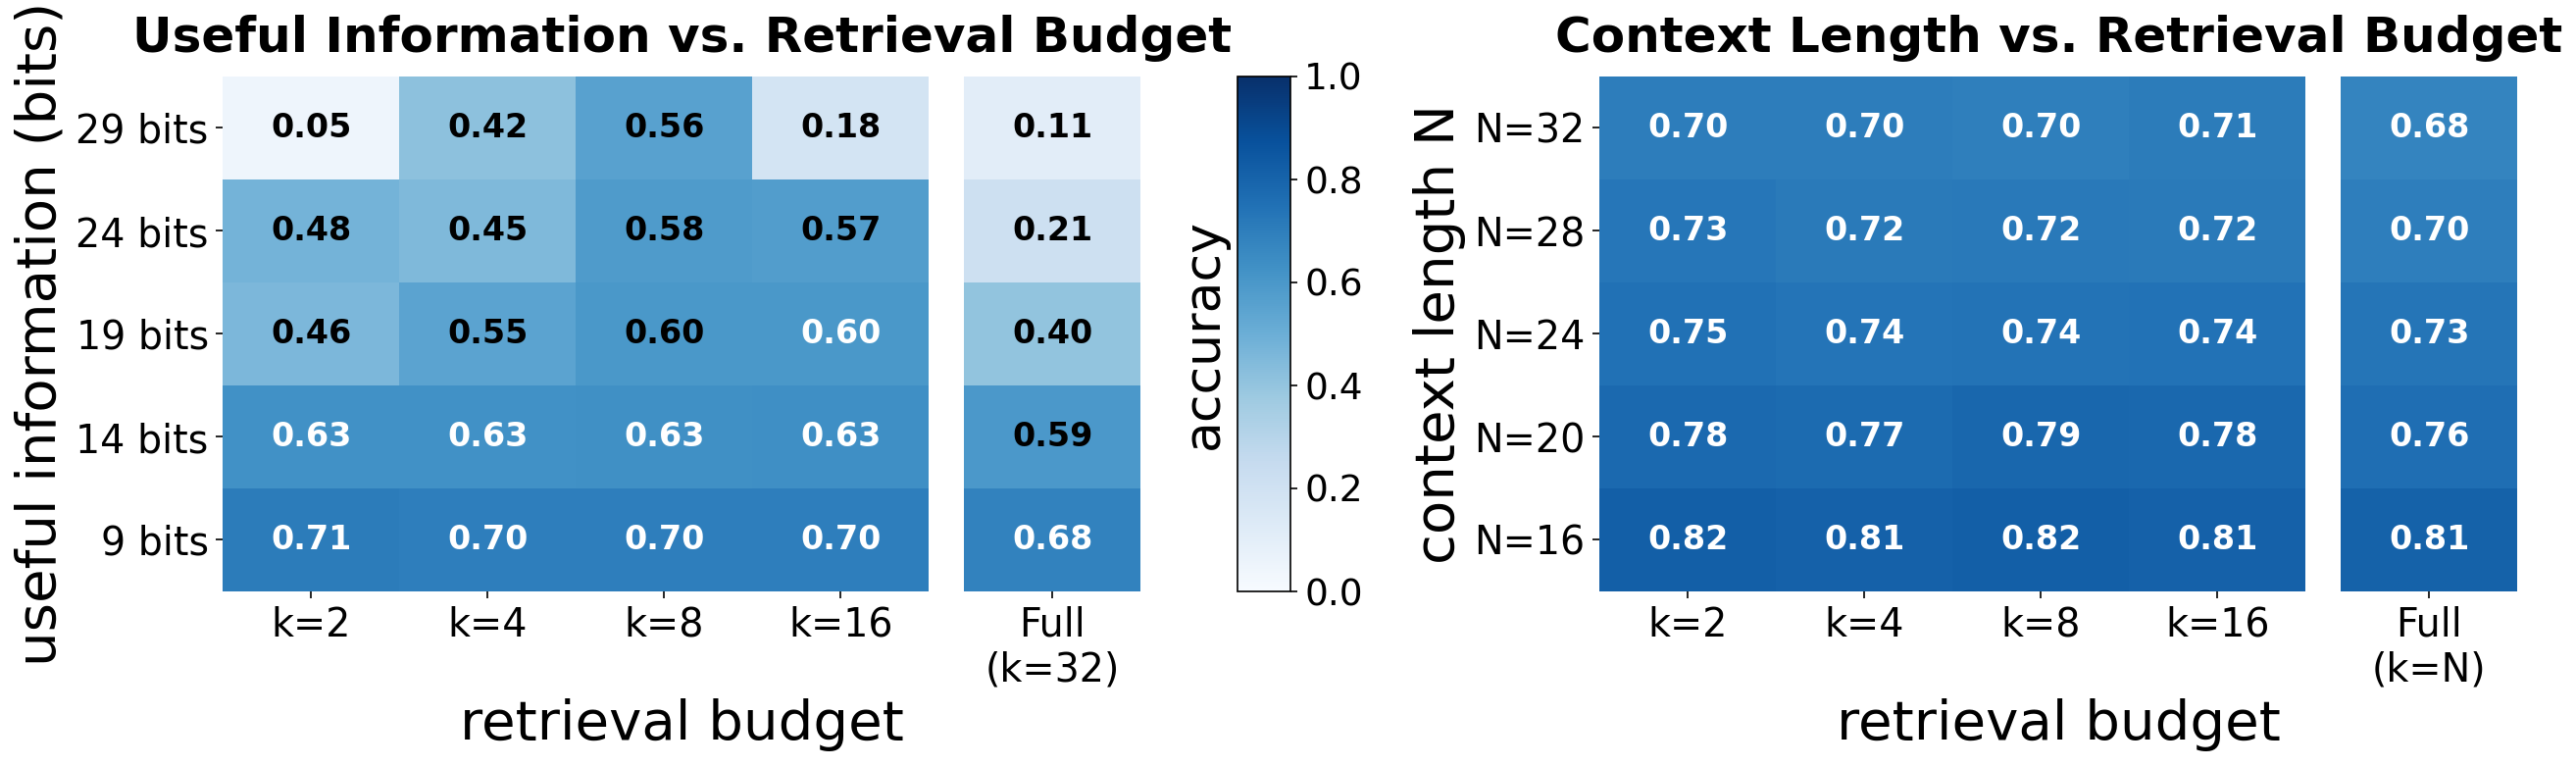
\includegraphics[width=\linewidth]{figures/k_vs_N_retrievalv2.png}
    \vspace{-0.84cm}
    \label{fig:k_ablation}
\end{figure}
We hypothesize that the retrieval budget $k$ should depend on the information required for a decision, rather than on the context length $N$. While isolating this in manipulation is non-trivial, we evaluate on a controlled toy dataset by varying the minimum bits of information required to make a prediction, and the context length $N$. We observe that for fixed $N$, performance is similar across $k$ values but varies across tasks with different information requirements.


\begin{figure*}[h]
    \centering
    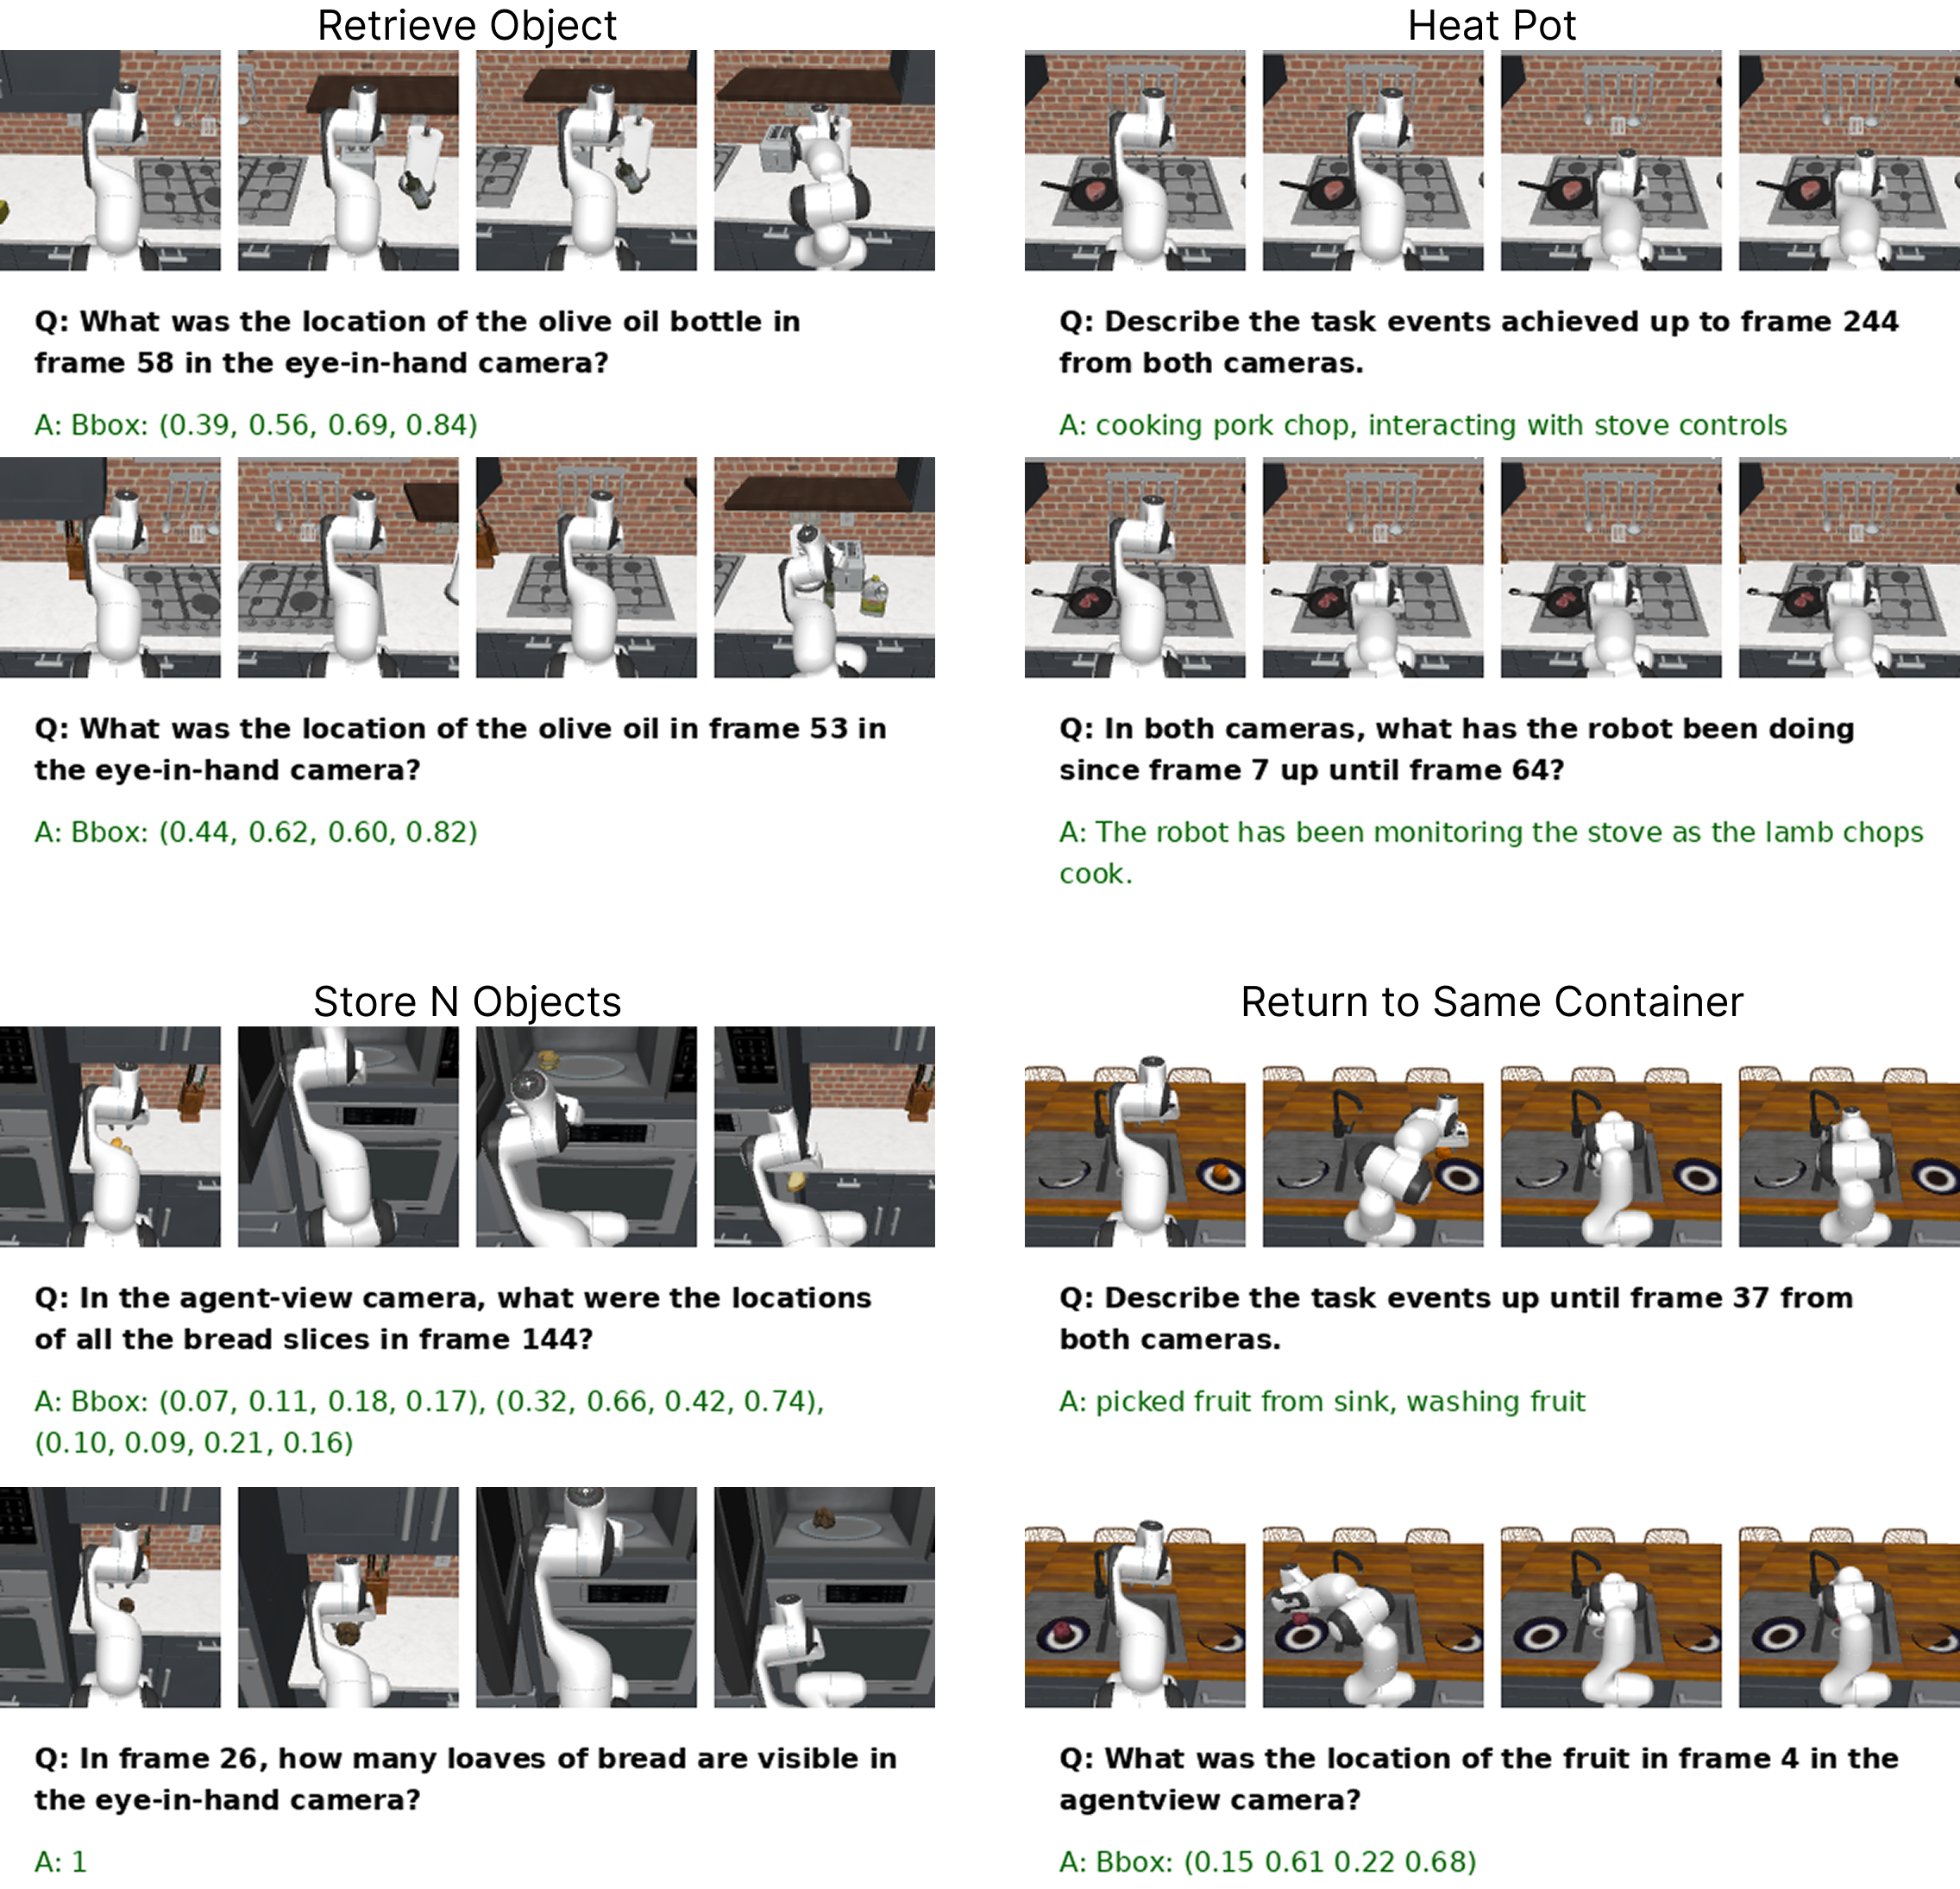
\includegraphics[width=\textwidth]{figures/qa_examples.png}
    \caption{Examples of automatically generated video question--answer pairs across tasks, illustrating different types of task-relevant information required to answer the queries. We only show four frames uniformly sampled from the video to maintain visual clarity.}
    \label{fig:qa_examples}
    \vspace{-0.5em}
\end{figure*}
\subsection{Implementation Details}\label{sec:impl}
\noindent
\textbf{Architecture.}
The observation encoder $g_\theta^{\text{obs}}$ consists of a pretrained, frozen vision model~\cite{crossmae} followed by a learned pooling layer that maps sensory inputs (e.g., RGB and proprioception) to a single embedding.
The action encoder $g_\theta^{\text{act}}$ embeds past actions using an MLP.
The policy backbone $f_\theta$ is a Transformer with $6$ layers of local attention with $4$ heads each, followed by $2$ layers that perform long-horizon retrieval using top-$k$ attention.
The action head $h_\theta^{\text{act}}$ is an MLP that predicts $32$ future actions, and the text head $h_\theta^{\text{text}}$ is a single Transformer block that autoregressively predicts answers over the standard Qwen3 vocabulary~\cite{qwen3}.
\\
\textbf{Top-$K$ attention.}
We maintain an explicit memory buffer $\mathcal{M}_t$ containing $192$--$768$ entries per episode, depending on the maximum task horizon.
Entries are added to the memory every $8$ interaction steps, and each entry stores either per-camera observation embeddings $x_i$ or past action embeddings $e_i$.
At each time step, top-$k$ attention selects $k=8$ entries based on cosine similarity.
We use a straight-through estimator to enable backpropagation through the top-$k$ selection.
\begin{table*}[h]
\centering
\caption{Task settings across simulation and real-world domains.}
\label{tab:task-settings}
\resizebox{0.75\textwidth}{!}{%
\begin{tabular}{lllll}
\toprule
\multirow{2}{*}{\textbf{Task Name}} 
& \multirow{2}{*}{\textbf{Domain}} 
& \multirow{2}{*}{\shortstack{\textbf{Max Memory} \\ \textbf{Storage}}}
& \multirow{2}{*}{\shortstack{\textbf{\# Cameras}}}
& \multirow{2}{*}{\shortstack{\textbf{\# Expert} \\ \textbf{Demos}}} \\
\\
\midrule
Retrieve Object & Simulation & $196$ & $2$ & $50$ \\
Retrieve Object & Real-world & $192$ & $1$ & $50$ \\
Return to Same Container & Simulation & $192$ & $2$ & $50$ \\
Return to Same Container & Real-world & $192$ & $2$ & $100$ \\
Store $N$ Objects & Simulation & $768$ & $2$ & $50$ \\
Store $N$ Objects & Real-world & $768$ & $2$ & $100$ \\
Heat Stove for $T$ mins & Simulation & $768$ & $2$ & $50$ \\
Heat Stove for $T$ mins & Real-world & $768$ & $2$ & $60$ \\
\bottomrule
\end{tabular}
}
\end{table*}
\\
\noindent
\textbf{Losses and weighting.}
The overall training objective is $\mathcal{L} = \mathcal{L}_{\text{IL}} + \lambda \mathcal{L}_{\text{VQA}}$, with $\lambda=1.0$.
For imitation learning, actions are optimized using an $\ell_1$ loss.
For VQA, answers are optimized using a cross-entropy loss.
\\
\textbf{VQA generation and filtering.}
Trajectory-to-text summaries are generated using SAM3~\cite{sam3} and gpt-4o-mini~\cite{gpt-4o}.
For each trajectory, we generate $20$ questions by randomly sampling frame indices and prompting GPT-4o-mini to produce corresponding $(u, v)$ pairs.
Generated pairs are filtered using gpt-4o~\cite{gpt-4o} as a judge model based on correctness and relevance. Both the prompts for generation and verification are provided in Sec.~\ref{sec:app:prompts}.
The final VQA dataset contains $20$k--$30$k question--answer pairs per task.
\\
\begin{table*}[h]
\centering
\caption{Training hyperparameters.}
\label{tab:training-config}
\resizebox{\columnwidth}{!}{%
\begin{tabular}{ll}
\toprule
\textbf{Config} & \textbf{Value} \\
\midrule
Optimizer & AdamW \\
Base learning rate & $5\times10^{-4}$ \\
Effective batch size & $32$ \\
Weight decay & $0.01$ \\
Warmup epochs & $2$ \\
Total epochs & $200$ \\
Early stopping epochs & $50$ \\
Action prediction horizon & $32$ \\
Proprioception noise (std) & $0.005$ \\
Brightness augmentation & $\mathrm{Uniform}(-0.1,\,0.1)$ \\
Contrast augmentation & $\mathrm{Uniform}(0.8,\,1.2)$ \\
\bottomrule
\end{tabular}
}
\end{table*}
\textbf{Training details.}
All models are trained end-to-end using the hyperparameters listed in Table~\ref{tab:training-config}, with separate models for each task.
\\
\textbf{Evaluation protocol.}
Policies are evaluated in a closed loop over $50$ episodes per task in simulation and $20$ episodes per task in the real world.
We report the final task success rate.


\subsection{Prompts}\label{sec:app:prompts}
Please see the bottom of the appendix.
\input{src/figures/prompts}